% This is samplepaper.tex, a sample chapter demonstrating the
% LLNCS macro package for Springer Computer Science proceedings;
% Version 2.20 of 2017/10/04
%
\documentclass[runningheads]{llncs}
%
\usepackage{graphicx}
% Used for displaying a sample figure. If possible, figure files should
% be included in EPS format.
%
% If you use the hyperref package, please uncomment the following line
% to display URLs in blue roman font according to Springer's eBook style:
% \renewcommand\UrlFont{\color{blue}\rmfamily}
\usepackage[numbers,sort&compress]{natbib}
\begin{document}
%
\title{Learning Spectral Representations:\\ Semantic Memory and the\\ Information Dynamics of Thinking}
%
\titlerunning{Learning Spectral Representations}
% If the paper title is too long for the running head, you can set
% an abbreviated paper title here
%
\author{Steve~Homer\inst{1}\orcidID{0000-1111-2222-3333} \and
Geraint~A.~Wiggins\inst{1,2}\orcidID{0000-0002-1587-112X}}
%
\authorrunning{S.~Homer and G.~A.~Wiggins}
% First names are abbreviated in the running head.
% If there are more than two authors, 'et al.' is used.
%
\institute{AI Lab, Vrije Universiteit Brussel, 1050 Brussels, Belgium \and
School of Electronic Engineering and Computer Science,\\Queen Mary University of London, Mile End Road, London E1 4FZ, UK \\
\email{steven.t.homer@gmail.com,geraint@ai.vub.ac.be}}
%
\maketitle              % typeset the header of the contribution
%
\begin{abstract}
The abstract should briefly summarize the contents of the paper in
150--250 words.

\keywords{Statistical learning  \and Representation Learning \and Information Dynamics.}
\end{abstract}
%
%
%
\section{Introduction}
This paper presents progress in statistical knowledge representation applied to auditory input, specifically speech. The work has been conducted in the context of a longer-term project, on the Information Dynamics of Thinking (IDyOT). Until the current publication, the work has focused either on theoretical explication \cite{Wiggins12,WigginsForth15,ForthAgresEtAl16,vanderVeldeForthEtAl17,Wiggins18}, or on statistical modelling applied to textual data \cite{WigginsSanjekdar19}. In this paper, we begin to explore the potential of the IDyOT theory to learn its own representations and build hierarchical ``deep'' representations of meaning. At this stage, we do not claim that these representations are cognitively valid; rather we attempt just to demonstrate that the proposal is capable of learning from data in the way proposed, and that the representations produced are credible as the output of a human-like learning system. The key contribution of the present paper is the use of spectral approaches to knowledge representation and the extraction of knowledge from time-variant speech information in the context of structural analysis by statistical model.

In the following sections, we first outline the context of the Information Dynamics of Thinking project, and summarise it. We then explain the detail of our implementation. We detail the empirical studies we have conducted to test whether the theory identifies perceptual and semantic categories as predicted. Finally, we discuss the prospects for future work on the model.
\section{Background}
\subsection{Overview}
\begin{figure}[t]
    \centering
    \resizebox{.9\linewidth}{!}{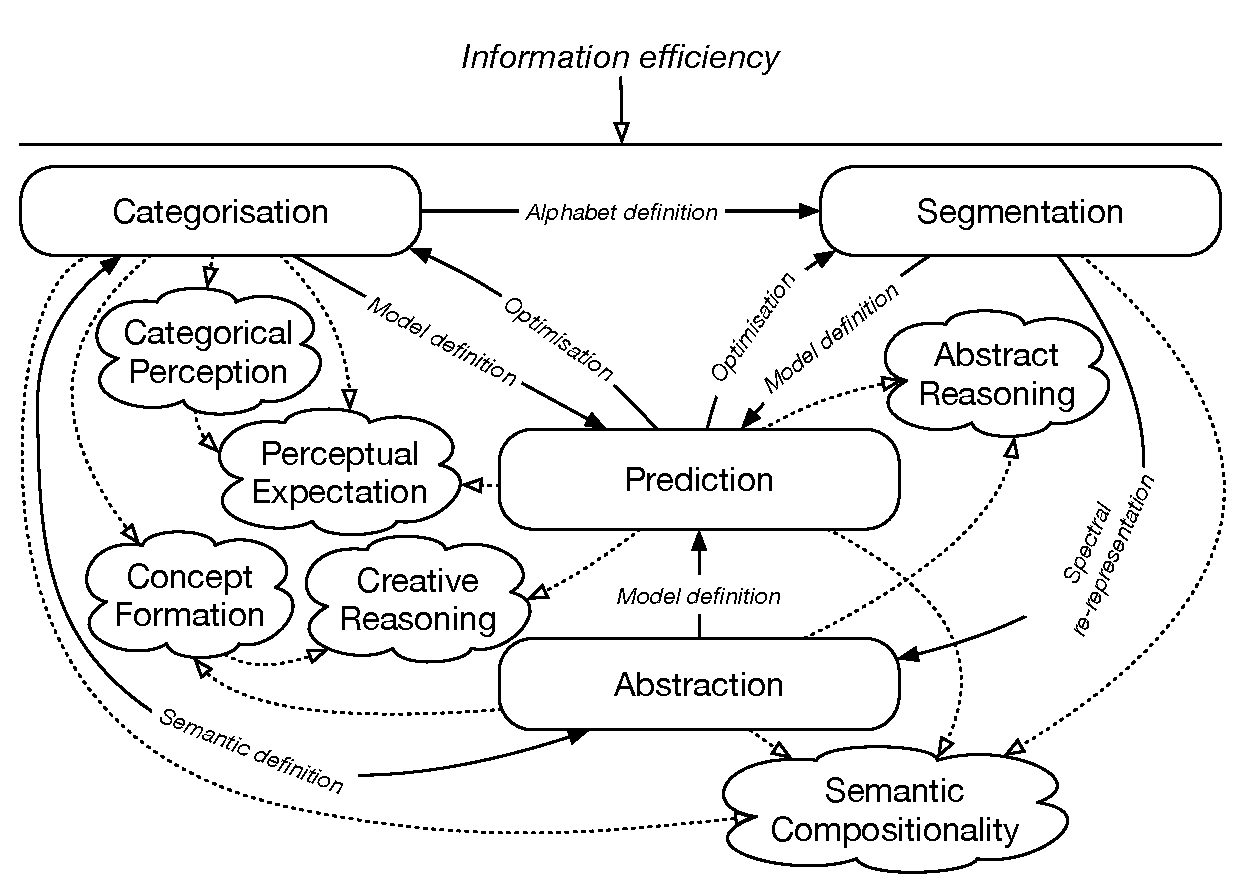
\includegraphics{pix/overview}}
    \caption{Overview of IDyOT components and operation cycle. Rounded boxes are the main IDyOT processes. Cloud shapes represent the phenomena explicated. Arrows are labelled with the operations that connect the main processes. The whole is guided by the information efficiency criterion. Figure and caption reproduced under CC-BY license \cite{WigginsSanjekdar19}.}
    \label{fig:IDyOToverview}
\end{figure}
The theory of Information Dynamics of Thinking (IDyOT) is an attempt to capture in an implemented computational model a hypothetical fundamental cognitive process. That process, it is claimed, drives cognition and action in a mind. The theory draws together the processes of (implicit, non-conscious) learning, segmentation of sequences in time, construction of categorical perceptual and semantic representations, and abstraction of data into ontological hierarchies. The motivation of the theory is to be able to predict what happens next in the world, so it accords mostly with the approach of Clark \cite{Clark13}. Like many such theories, it is based on statistical modelling (viewed as a simulation of cognitive process, not as a model of data) and Shannon information theory \citep{Shannon48}. The theory is formulated as one of ``information dynamics'', and not as one of ``free energy''  \citep{Friston10}, because there is evidence (from music cognition studies  \citep{Huron06,PearceWiggins12,HansenPearce14}) that humans are directly sensitive to the quantity of Shannon entropy in perceived data, and so  grander physical metaphor is superfluous.

The IDyOT process is illustrated in Fig.~\ref{fig:IDyOToverview}. It operates over 
% this bit taken directly from Frontiers paper - needs reworking
input sequences at a given basic level of representation---here, the vectors of a Fourier Transform of human speech. These sequences are segmented using boundary entropy \cite{SproatShihEtAl94}, which we explain below. Each segment so produced is then represented as a temporal trajectory in a geometrical space of dimension and scale appropriate to its particular input type.  This space becomes the semantic space of the data level with which it is associated. As the sequence is so segmented and recorded, a superordinate sequential and semantic layer is constructed, from vectors determined by spectral transforms of the multidimensional sequences at the subordinate layer. The representations are spectral because this mathematical approach allows comparison of sequences of varying lengths, each represented by a single point in the superordinate space; in our case, the spectral transformation is the standard Fourier Transform \cite{?}. In the current initial experiments, the geometry of the superordinate space is Euclidean. However, in general, that geometry is constructed by an inner product function that induces a norm (distance) that models similarity in this particular space.

The whole process is guided by an information efficiency criterion, expressed domain-independently in terms of a Shannon-type estimate of the average number of bits required to represent each symbol in the learned memory. In what follows, we refer to this quantity as {\it mean information content}; the estimated number of bits to required to represent a signal is called the {\it information content}.




\subsection{Perceptual Segmentation by Boundary Entropy}
\subsection{Conceptual Spaces}
\cite{Gardenfors00,Gardenfors14}
\subsection{Spectral Representations of Meaning}
\cite[][\S7.2.5]{Wiggins18}
\subsection{The Information Dynamics of Thinking}

\paragraph{Segmentation}
\paragraph{Categorisation}
\paragraph{Abstraction}
\paragraph{Prediction}

\section{Implemented Model}
{\it Steve to do from here on...}
\section{Experiments}
\subsection{Data}
\subsection{Results}
\section{Discussion}
\section{Conclusion and Future Work}

% ---- Bibliography ----
%
% BibTeX users should specify bibliography style 'splncs04'.
% References will then be sorted and formatted in the correct style.
%

\bibliographystyle{splncs04}
\bibliography{BibDesk}
%

\end{document}
